\section{Dataset}
\label{sec:meth}
\subsection{Data Source}
VirusTotal~\cite{virustotal} is a free online service that analyzes whether files submitted by real-world users are malwares. It can identify  a large variety of malwares such as viruses, worms, and trojans. For each submitted file, VirusTotal applies different antivirus engines to detect and finally generates an aggregated report. In the report, each antivirus engine would give a result whether the file is malicious and tag a \emph{malware family} to the file if it is malicious. \wenfei{define malware family here.} All submitted files and generated reports are saved and can be accessed through public API, and they are viewed as malware repository. VirusTotal has been widely used by antivirus vendors to identify the effectiveness of their products. That is, they can submit suspicious files compare the identification results of their products with other vendors, and thus to know the false negatives and false positives of their products.


The repository on VirusTotal provides a good source for characterizing malwares. Firstly, the data on VirusTotal covers vast majority of malwares in the real world.
Figure~\ref{fig:subnum} shows that there were more than 40 million suspicious files submitted last November. 
This huge amount of data is a rough estimation of malwares in the real world. \wenfei{need supporting reference.}
Secondly, all submitted files on VirusTotal are already analyzed and labeled by state-of-the-art antivirus techniques. VirusTotal updates each antivirus engine every 5 minutes. For each submitted file, ViruaTotal keeps both the identification result (i.e. whether the file is malware) and the exact detection tag returned by each engine. To complement the results for antivirus engines, malware researchers can comment and vote each submitted file. Thus, we believe mining the characteristics of data on VirusTotal could lead to representative results for a large variety of application (e.g., ``Big Security"). \wenfei{BTW, what is Big Security?}

\wenfei{put this to related work.}In academia, researchers began to pay attention to mining VirusTotal repository. 
For example, ~\citet{neeles} leverage submission\_id information to identify malware writers, 
who use VirusTotal as a test platform. 
We believe there are much more research opportunities through mining VirusTotal. 

\subsection{Data Collection}
\begin{table}[h!]
\centering
\footnotesize
{
%\begin{tabular}{@{\hspace{3pt}}l@{\hspace{3pt}}|@{\hspace{3pt}}c@{\hspace{3pt}}}
\begin{tabular}{l|l}
\hline
Metadata Fields & Explanation \\
\hline                            
%\cline{1-1}
{\bf name}      & file name of the submitted sample \\
{\bf timestamp} & timestamp when the submission is conducted \\
{\bf source\_country} & the country where the submission is conducted \\
{\bf source\_id} & user id who conducts the submission\\
{\bf tags} & VirusTotal tag \\
{\bf link} & where to download the submitted sample \\
{\bf size} & file size \\
{\bf type} & file type \\
{\bf first\_seen} & when the same sample was first submitted \\
{\bf last\_seen} & when the same sample was last submitted \\
{\bf hashes} & including sha1, sha256, vhash, md5, and ssdeep\\
{\bf total} & how many engines analyze the sample\\
{\bf positives} & how many engines identify the sample as malicious \\
{\bf positives\_delta} & changes about {\bf positives} fields \\
{\bf report} & detailed detection report from each AV engine \\
%\multicolumn{2}{|l|}
\hline

\end{tabular}
}
\caption{Metadata fields of each submission got from VirusTotal private API.}
\label{tab:fields}
\end{table}


We download submission reports' metadata through private API of VirusTotal. 
Table~\ref{tab:fields} shows all metadata fields and their meaning. 
It is possible that VirusTotal private API returns redundant reports, 
and we use the combination of md5 and timestamp
 to detect and merge redundant reports.

\begin{figure}[t!]
\begin{center}
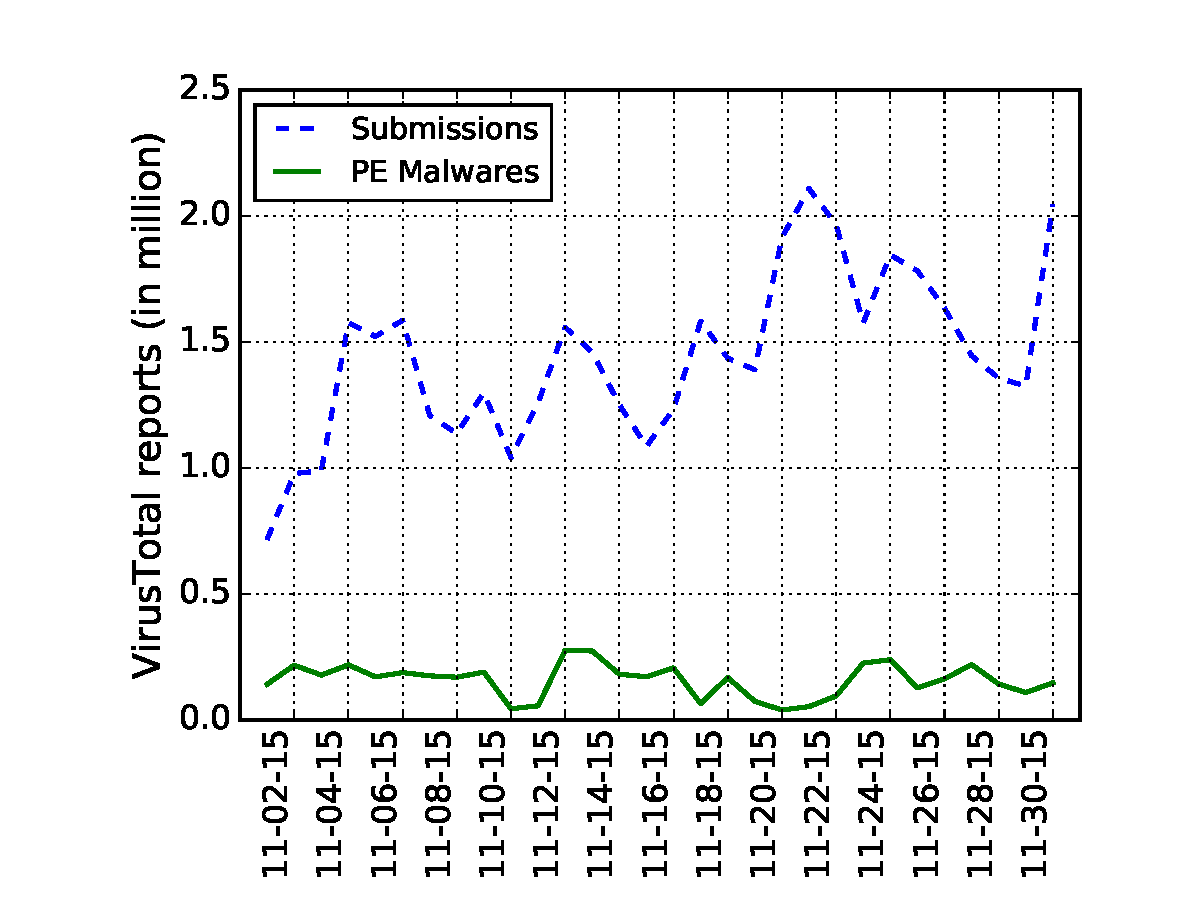
\includegraphics[width=2.5in]{figure/nov}
\caption{The number of suspicious files and the number of malwares submitted to VirusTotal in November of 2015. }
\label{fig:subnum}
\end{center}
\end{figure}

To guarantee analytic accuracy, we only focus on Portable Executable (PE) files, 
and we leave the analysis of other types of malicious files in the future. 
We filter all records by the tag field. If the tag field contains a ``peexe'' or ``pedll'', the record is considered as a PE file. 
Then we rely on Microsoft antivirus engine to judge whether the PE file is a malware and its malware family.
Among the 43 million downloaded reports in November 2015, 4.7 million of them are PE malwares. 
The numbers of reports and PE malwares submitted each day are shown in Figure~\ref{fig:subnum}.

After removing redundancy, we find that most malwares are submitted only once to VirusTotal. 4 million out of the total 4.7 million PE malware submissions are distinct. On average, each PE malware is submitted 1.17 times to VirusTotal. We believe that most malwares are encountered by more than one VirusTotal user. One possible reason of this observation is that VirusTotal users 
tend to check whether their samples have already been submitted, 
before conducting their submissions.

\textit{\underline{Threats to Validity.}}
Similar to all previous empirical study works, all our findings, experimental results, 
and conclusions need to be considered with our methodology in mind. 

VirusTotal private API only tracks which submission reports are sent to each downloader approximately, 
and there is no guarantee that all submission reports on VirusTotal can be downloaded successfully. 
It could be possible that we miss some malwares submitted to VirusTotal. 
We simply leverage Microsoft antivirus engine to decide whether one submission is malicious or not, 
and it is possible that Microsoft antivirus engine cannot make this decision precisely. 
However, how to get a precise label for a PE file is out of scope of this paper.  
Although there are huge mount of malwares on VirusTotal, we do believe that there are malwares never submitted to VirusTotal, 
and there are malwares submitted much later than when they appear in the real world.
However, there are no conceivable ways to study these malwares. 
We believe that malwares in our study provide a representative malware sample of the real world. 


